% This must be in the first 5 lines to tell arXiv to use pdfLaTeX, which is strongly recommended.
\pdfoutput=1
% In particular, the hyperref package requires pdfLaTeX in order to break URLs across lines.

\documentclass[11pt]{article}

% Remove the "review" option to generate the final version.
\usepackage[]{naacl2021}
% Standard package includes
\usepackage{times}
\usepackage{latexsym}

% For proper rendering and hyphenation of words containing Latin characters (including in bib files)
\usepackage[T1]{fontenc}
% For Vietnamese characters
% \usepackage[T5]{fontenc}
% See https://www.latex-project.org/help/documentation/encguide.pdf for other character sets

% This assumes your files are encoded as UTF8
\usepackage[utf8]{inputenc}

% This is not strictly necessary, and may be commented out,
% but it will improve the layout of the manuscript,
% and will typically save some space.
\usepackage{microtype}

% If the title and author information does not fit in the area allocated, uncomment the following
%
%\setlength\titlebox{<dim>}
%
% and set <dim> to something 5cm or larger.

\renewcommand{\UrlFont}{\ttfamily\small}
\usepackage{multirow}
\usepackage{amsmath}
\usepackage{amsfonts}
\usepackage{colortbl}
\usepackage{graphicx, subfigure}

% add color to table
\usepackage{xcolor,colortbl}

\newcommand\BibTeX{B\textsc{ib}\TeX}
\newcommand{\modelname}{\textsc{Entailment}}
\newcommand{\hybrid}{\textsc{Hybrid}}
\newcommand{\intentdata}{\textsc{IFS-Intent}}
\newcommand{\relationdata}{\textsc{IFS-Relation}}
\newcommand{\yihao}[1]{\textcolor{red}{#1}}



\title{Incremental Few-shot Text Classification with Multi-round New Classes:\\Formulation, Dataset and System}

% Author information can be set in various styles:
% For several authors from the same institution:
% \author{Author 1 \and ... \and Author n \\
%         Address line \\ ... \\ Address line}
% if the names do not fit well on one line use
%         Author 1 \\ {\bf Author 2} \\ ... \\ {\bf Author n} \\
% For authors from different institutions:
% \author{Author 1 \\ Address line \\  ... \\ Address line
%         \And  ... \And
%         Author n \\ Address line \\ ... \\ Address line}
% To start a seperate ``row'' of authors use \AND, as in
% \author{Author 1 \\ Address line \\  ... \\ Address line
%         \AND
%         Author 2 \\ Address line \\ ... \\ Address line \And
%         Author 3 \\ Address line \\ ... \\ Address line}

\author{Congying Xia$^{1}$\thanks{~ Indicates Equal Contribution.}, Wenpeng Yin${^2\footnotemark[1]}$, Yihao Feng$^{3}$, Philip Yu$^{1}$\\
{$^1$University of Illinois at Chicago, Chicago, IL, USA} \\
{$^2$Salesforce Research, Palo Alto, CA, USA} \\
{$^3$University of Texas at Austin, Austin, TX, USA} \\
 {\tt \{cxia8, psyu\}@uic.edu},
 {\tt wyin@salesforce.com},
 {\tt yihao@cs.utexas.edu}
 }

\begin{document}
\maketitle
\begin{abstract}
%Text classification is usually studied by from a pre-defining the range of classes. In the real-world, new classes might keep challenging the existing system while limited examples are available. An intelligent system should be able to recognize upcoming new classes with a few examples.
%% Text classification is usually studied by labeling natural language texts with relevant categories from a predefined set. In the real-world, new classes might keep challenging the existing system with limited labeled data. The system should be intelligent enough to recognize upcoming new classes with a few examples. In this work, we define a new task in the NLP domain---``incremental few-shot text classification'', where the system first handles some base classes with rich annotations, then copes with multiple rounds of new classes.
%For each round, there are a small group of new classes, each with merely a few labeled examples. There are two main challenges for this new problem:  
%%For each round, there is a batch of new classes with a few labeled examples per class. Two major challenges are existing in this new task: (i) For the learning process, the system should incrementally learn new classes round by round without re-training on the examples of preceding classes; (ii) For the performance, the system should perform well on new classes without much loss on preceding classes. In addition to formalizing the new task, we also release two benchmark datasets in the incremental few-shot setting: intent classification and relation classification. Moreover, we propose an approach \modelname, which shows promise for solving this novel problem.

Text classification is usually studied by labeling natural language texts with relevant categories from a predefined set. In the real world, new classes might keep challenging the existing system with limited labeled data. The system should be intelligent enough to recognize upcoming new classes with a few examples. In this work, we define a new task in the NLP domain, \textit{incremental few-shot text classification}, where the system incrementally handles multiple rounds of new classes. For each round, there is a batch of new classes with a few labeled examples per class. Two major challenges exist in this new task: (i) For the learning process, the system should incrementally learn new classes round by round without re-training on the examples of preceding classes; (ii) For the performance, the system should perform well on new classes without much loss on preceding classes. In addition to formulating the new task, we also release two benchmark datasets \footnote{Code \& Data are available at \url{https://github.com/congyingxia/IncrementalFSTC}.} 
in the incremental few-shot setting: intent classification and relation classification. Moreover, we propose two entailment approaches, \modelname\enspace and \hybrid, which show promise for solving this novel problem.
\end{abstract}


\section{Introduction}
%Supervised text classification has achieved great success in the past decades due to the availability of rich training data and deep learning techniques. Few-shot text classification is also attracting increasing attention from the community because we realize that it is unlikely to have large-scalar labeled data for new classes in reality. 
Text classification has achieved great success in the past decades with the development of deep learning techniques \cite{kowsari2019text, li2020survey}. However, decent performance highly relies on the availability of large-scale task-specific training data. Recently, few-shot text classification \cite{yu2018diverse, geng2019induction, xia2020composed} has attracted increasing attention from the NLP community since it is unlikely to have large-scale labeled data for new classes in the real world. 

Typically, few-shot text classification is formulated like this: the system first sees a set of base classes $C_b$ that have a large number of labeled examples,
%then the system is provided a group of new classes $C_n$, each of which has $k$ examples only.
then a group of new classes $C_n$ is provided with $k$ examples per class.
For a testing instance, the system is required to search for its label in the space of $C_b\cup C_n$ or merely $C_n$. However, this setting might not suitable for real scenarios. First, base classes with rich annotations might not be available at the beginning. It happens whenever you want to build a system from scratch. Second, take the bank's customer service system as an example, queries with new intents are continuously appearing (e.g., by a sequence of rounds) without enough labeled data. The system should be able to keep learning and recognizing new intents round by round. For each query, the system needs to pick up the most appropriate intent in the incrementally increasing label space or return ``none of them''.
%from either $C_b\cup C_n$ or merely $C_n$.

%However, if we think about the real-world application of few-shot text classification, new  challenges exist and need our exploration. First, take the bank's customer service system as an example, new intents might be expressed to an existing system gradually (e.g., by a sequence of rounds) while no much-labeled data can be provided. The system should be able to keep learning and recognizing new classes round by round. For a new customer's request, the system need to pick up the most appropriate intent from all seen intents or return ``none of them''. Second, existing training strategies tend to make the system forget what it has learnt in the past while fine-tuning on some new data. So, if we directly fine-tune a system on the new rounds of classes, the system's performance on the old classes will drop dramatically. For a real-world application, such as the aforementioned customer service system, we definitely want the system to perform well on all classes, regardless of when the system sees the class and how many examples are associated with.
%%However, if we think about few-shot text classification in real scenarios, new challenges exist which makes it worth further exploration. First, take the bank's customer service system as an example, queries with new intents are continuously appearing, (e.g., by a sequence of rounds), without enough labeled data. The system should be able to keep learning and recognizing new intents round by round. For each query, the system needs to pick up the most appropriate intent in the incrementally increasing label space or return ``none of them''. Second, existing incremental training strategies have the problem of catastrophic forgetting \cite{mccloskey1989catastrophic}. The systems tend to forget the knowledge learned in the past when continually fine-tuning on new classes. This leads to a significant drop in the performance of base classes. For a real-world application, such as the aforementioned customer service system, the system is expected to perform well on all classes, regardless of when the classes come to the system or how many examples they have.



% there are new challenges exist in real scenarios for few-shot text classification.
%if we think about few-shot text classification in real scenarios, new challenges exist and make it worth further exploration. 

In this work,
%our contribution lies in three aspects. First, 
we propose a more realistic and challenging task in the low resource scenarios: \textit{incremental few-shot text classification}. In this new task, the system is provided with $m$ rounds of new classes (i.e., $C^1_n$, $C^2_n$, $\cdots$, $C^m_n$) without any base classes that have enough annotations. For each round, there are a group of new classes, $C^i_n$ ($i=1, \cdots, m$), and each class has $k$ labeled examples ($k$ is in the range of [1, 5] and varies for different classes). During testing, the system is required to either select the best class from $C^1_n \cup C^1_n\cdots \cup C^m_n$ or output ``none of them'' which means no existing class applies to the input. As far as we know, this is the first work that studies incremental few-shot learning without base classes. All previous few-shot learning models \cite{DBLPSnellSZ17, DBLPGidarisK18, yin2020universal, xia2020cg, nguyen2020semantic} fail to solve this problem since they relied on the large-scale labeled data of base classes to train a robust system. To provide a complete vision about incremental few-shot text classification, we also conduct experiments with additional base classes to compare with these baselines.

%%In this work, our contribution lies in three aspects. First, we formally define this problem: ``incremental few-shot text classification''. In our definition, the system is first provided with some base classes $C_b$ with rich annotations, then $m$ rounds of new classes (i.e., $C^1_n$, $C^2_n$, $\cdots$, $C^m_n$) will come sequentially. Each $C^i_n$ ($i=1, \cdots, m$) consists of a group of new classes and each class has $k$ labeled examples ($k$ is in the range of [1, 5] and varies for different classes). For testing, we require the system to either select the best class from $C_b\cup C^1_n \cup C^1_n\cdots \cup C^m_n$ or output ``none of them'' which means no existing class applies to the input. As far as we know, this is the first work in the NLP community that studies text classification with an incremental size of classes. There are a few papers working on incremental few-shot classification in the field of computer vision \cite{DBLPRenLFZ19}. However, they only consider one round of new classes. It's difficult to evaluate the system's ability for incremental learning without multi-rounds of new classes.
%It makes difficulties to check if and how much the system's performance will drop with more rounds of new classes. 

%Second, we build two benchmark datasets for this new problem. One is intent classification which simulates a task like the bank's customer service we just mentioned. The other is relation extraction. Existing relation extraction tasks always have a fixed-size of relation types. In reality, the relations we are interested in are much more than the ones covered in some datasets. For example, we may want to detect some fine-grained relations or implicit relations that need entailment. We cannot expect the availability of large-scale training data for open-domain, open-form relations. In our benchmark, we first provide some relations as base classes, then let new classes come in as groups gradually. This goes from the popular multi-class relation classification to the open relation classification with a few-shot setting. Apart from above feature in the training set, another important feature of our benchmark datasets is that we do not provide dev sets. Existing systems are commonly evaluated on the dev set and finally only the best dev model is kept. We claim that in real-world (incremental) few-shot applications, we cannot expect extra labeled data other than the $k$ examples. This is in line with the observation in \cite{DBLP07676}. If a system has to rely on dev set to find the best parameters, it cannot be applied to incremental few-shot problems.

%% Furthermore, we consider an extreme case where no base classes are available. This situation is named as incremental few-shot text classification without base classes. It happens whenever you want to build a system from scratch. In real-world scenarios, base classes with rich annotations might not be available at the beginning. In this setting, we need to solve the cold start problem where no initial annotations are available. All previous few-shot learning models \cite{DBLPSnellSZ17, DBLPGidarisK18, DBLPRenLFZ19} fail to solve this problem, since they relied on the large-scale labeled data for base classes to train a robust system. 

%%% Second, to evaluate the aforementioned two settings, incremental few-shot text classification with/without base classes, we release a benchmark dataset, \intentdata\enspace for evaluation. This benchmark simulates a task like the bank's customer service as we just mentioned. Another important feature of our benchmark datasets is that we do not provide dev sets. Existing systems are commonly evaluated on the dev set to choose the best training model. We claim that in real-world (incremental) few-shot applications, we cannot expect extra labeled data other than the $k$ examples. This is in line with the observation in \citet{DBLP07676}. If a system has to rely on dev set to find the best parameters, it is not suitable for the incremental few-shot setting.

%%Second, we build two benchmark datasets for this new problem. One is intent detection that aims at understanding the intents under user queries \cite{liu2016attention}. This benchmark simulates a task like the bank's customer service as we just mentioned. The other is relation classification which needs to determine the correct relation between two entities in a given sentence \cite{zeng2014relation}. In reality, the relation types might be unlimited. For example, there are fine-grained relations or implicit relations that need entailment. In open-domain or open-form relation tasks, there always exist the problem of lack of annotations. In these two benchmark datasets, we first provide some intents/relations with enough training data as base classes. Then, new classes with a few examples are added into the system round by round. 

To evaluate the performance for different models, we build two benchmark datasets for this new problem. One is intent detection that aims at understanding the intents under user queries \cite{liu2016attention, xia2018zero}. This benchmark simulates a task like a bank's customer service as we mentioned. The other is relation classification which needs to determine the correct relation between two entities in a given sentence \cite{zeng2014relation}. In reality, the relation types might be unlimited. For example, there are fine-grained relations or implicit relations that need entailment. In open-domain or open-form relation tasks, there always exists the problem of lack of annotations. 

Another important feature of our benchmark datasets is that we do not provide dev sets. Existing systems are commonly evaluated on the dev set to choose the best training model. We claim that in real-world (incremental) few-shot applications, we cannot expect extra labeled data other than the $k$ examples. This is in line with the observation in \citet{DBLP07676}. If a system has to rely on the dev set to find the best parameters, it is not suitable for the incremental few-shot setting.

%In these two benchmark datasets, we first provide some intents/relations with enough training data as base classes. Then, new classes with a few examples are added into the system round by round. 


%%Third, we propose our approach, \modelname, to solve this new problem. \modelname\enspace models the text classification problem as a textual entailment \cite{dagan2013recognizing} problem. To figure out if an input $x$ belongs to a class $y$, \modelname\enspace tries to infer the truth value of $y$ (i.e., a hypothesis), given the $x$ (i.e, the premise). The main benefit of this formulation is that the system learns this task not only from  the label-specific examples, but more importantly, from the large-scale entailment datasets. In other words, we make use of indirect supervision from textual entailment datasets to address the target few-shot task. Specifically, for each round $C_n^i$ which has $h$ new classes with $k$ examples for each, we first build positive (premise, hypothesis) pairs by accompanying each input with its gold class, and negative (premise, hypothesis) pairs by accompanying the input with other $h-1$ classes in $C_n^i$. It is worth noting that we only use the few-shot examples and label names in $C_n^i$ for the incremental training.

Furthermore, we propose a novel approach, \modelname, to solve this new problem. \modelname\enspace models the text classification problem in a textual entailment \cite{dagan2013recognizing} framework. To figure out if an input $x$ belongs to a class $y$, \modelname\enspace tries to infer the truth value of $y$ (i.e., a hypothesis), given the $x$ (i.e, the premise). The main benefit of this formulation is that the system learns this task not only from label-specific examples, but more importantly, from the large-scale entailment datasets. In other words, we make use of indirect supervision from textual entailment datasets to address the target few-shot task. 

In summary, our contribution lies in three aspects. 1) We propose a new task named Incremental Few shot Text Classification with multi-round new classes. This task is more challenging and realistic for low resource scenarios. 2) We create and release two benchmark datasets to evaluate the performance of this new task. 3) We propose two novel models, \modelname\enspace and \hybrid, to solve this novel problem. Extensive experiments on these two datasets show the effectiveness of our proposed models.
%The current state-of-the-art paper \cite{zhangdiscriminative} proposes a clustering-based model, DNNC, for few-shot text classification.  Instead of inferring the truth value of a class $y$ conditioned on the input text $x$, they tried to infer whether two text inputs ($x_i, x_j$) belong to the same class. In this way, the computation cost increased a lot since the number of examples is much more than the number of labels. The other issue is that their performance highly depends on the examples they choose. Additionally, we want to explore more possibilities and propose a hybrid entailment model, \hybrid, that combines the previous two methods. \hybrid\enspace utilizes entailment pairs from both \modelname\enspace and DNNC to train the entailment model.
%The other thing is that their final predictions need to be made by search the nearest neighbor among all the examples. The performance highly depends on the examples they choose. Bad examples will definitely bring poor results. 

%% Current state-of-the-art paper \cite{zhangdiscriminative} for few-shot text classification also utilizes textual entailment for pre-training. However, they ignore the information in the class labels. Instead of inferring the truth value of a class $y$ conditioned on the input text $x$, they tried to infer whether two text inputs ($x_i, x_j$) are in the same class. In this way, they not only increase the computation cost since the number of examples is much more than the number of labels. The other thing is that their final predictions need to be made by search the nearest neighbor among all the examples. The performance highly depends on the examples they choose. Bad examples will definitely bring poor results. 

%%our approach, \modelname, to solve this new problem. \modelname\enspace models the text classification problem as a textual entailment \cite{dagan2013recognizing} problem. To figure out if an input $x$ belongs to a class $y$, \modelname\enspace tries to infer the truth value of $y$ (i.e., a hypothesis), given the $x$ (i.e, the premise). The main benefit of this formulation is that the system learns this task not only from  the label-specific examples, but more importantly, from the large-scale entailment datasets. In other words, we make use of indirect supervision from textual entailment datasets to address the target few-shot task. Specifically, for each round $C_n^i$ which has $h$ new classes with $k$ examples for each, we first build positive (premise, hypothesis) pairs by accompanying each input with its gold class, and negative (premise, hypothesis) pairs by accompanying the input with other $h-1$ classes in $C_n^i$. It is worth noting that we only use the few-shot examples and label names in $C_n^i$ for the incremental training.

%%Current state-of-the-art paper \cite{zhangdiscriminative} for few-shot text classification also utilizes textual entailment for pre-training. However, they ignore the information in the class labels. Instead of inferring the truth value of a class $y$ conditioned on the input text $x$, they tried to infer whether two text inputs ($x_i, x_j$) are in the same class. In this way, they not only increase the computation cost since the number of examples is much more than the number of labels. The other thing is that their final predictions need to be made by search the nearest neighbor among all the examples. The performance highly depends on the examples they choose. Bad examples will definitely bring poor results. 




%%Usually, we can fine-tune the system on those positive/negative pairs to recognize the new classes in $C_n^i$. However, the fine-tuning process on new classes will lead to the forgetting of preceding classes. To mitigate the catastrophic forgetting problem \cite{mccloskey1989catastrophic}, we design a reminder mechanism: for an input in $C_n^i$, a preceding class still can be true and its probability of being true is dependent on how relevant it is to the new classes in $C_n^i$. Our reminder mechanism builds connections between the preceding classes and the new classes. It spreads some positive probabilities to the preceding classes so that the model can still remember the preceding classes while fine-tuning on the data of new classes. It is worth noting that we only use the few-shot examples in $C_n^i$ for the incremental training; meanwhile, the names of all the preceding classes are stored for the reminder mechanism.





\section{Related Work}
\label{sec:relatedwork}
\paragraph{Incremental few-shot learning.} As far as we know, there is no prior work in the NLP domain that studies incremental few-shot text classification. In this section, we mainly introduce some work in the computer vision domain. These works only assume that a single round of new classes $C_n$ is appended to the base classes $C_b$. Generally, they will learn class representations for classification.
%As we mentioned before, they only assume that a single round of new classes $C_n$ is appended to the base classes $C_b$. Generally, they will learn class representations for classification.
Different approaches differ in the way of representing base classes and new classes. Hereafter, we use $W_b$ and $W_n$ as the representations for $C_b$ and $C_n$, respectively.

%Hereafter, we use $W_b\in\mathbb{R}^{b\times d}$ and $W_n\in\mathbb{R}^{h\times d}$ as the representations for $C_b$ and $C_n$, respectively.

%\newcite{DBLPSnellSZ17} proposed Prototypical Network, in which both $W_b$ and $W_n$ are stored as the average representation of all images seen so far that belong to a certain class. Although Prototypical Network  was not for incremental few-shot learning, it can be easily applied to incremental problem as it only trains a nearest neighbor algorithm on the base classes and tests directly on the union of base and novel classes.
\newcite{DBLPSnellSZ17} proposes the Prototypical Network, in which both $W_b$ and $W_n$ are stored as the average embedding of the few-shot support images for a certain class.
Although Prototypical Network was not designed for incremental few-shot learning, it can be easily adapted to the incremental setting by providing the representations for all the classes. It trains a nearest neighbor algorithm on the base classes and tests directly on the union of base and new classes. \newcite{DBLPQiBL18} proposes an ``imprinting'' mechanism: the base representations $W_b$ are learned through supervised pre-training (e.g., the weight matrix in a softmax classifier), and $W_n$ are computed using the averaged representations like Prototypical Network.

% \textcolor{red}{Both the above methods do not incorporate base class information into novel class representations}.

In \citet{DBLPGidarisK18}, the base representations $W_b$ are learned through supervised pre-training. The representation of the $i^{th}$ novel class ($W_{n,i}$) comes from two origins: (i) the prototypical averaging, $w_{avg}$; (ii) attention-weighted sum over base representations: $w_{att}$. Namely,  $W_{n,i}=\phi_{avg}\odot w_{avg}+\phi_{att}\odot w_{att}$, where $\phi_{avg}$ and $\phi_{att}$ are learnable weight vectors. In the few-shot training stage, the original base classes $C_b$ are split into ``new base classes'' and ``fake novel classes'' for each episode. In testing, the representations of novel classes, $W_n$, are constructed based on the $k$ examples and $W_b$.

%The loss is computed when the system predicts ``new base classes'' as well as ``fake novel classes''. 

% Feature extractor and W\_base are trained in the 1st training stage. In the 2nd training stage, feature extractor is freezed, only W\_base and few-shot classification weight generator are trained. The difference between dynamic and prototypical is two fold. First, dynamic use ``cosine similarity'' to measure the query example and each class representation while prototypical use ``euclidean distance''. Second, dynamic use the attention between the base classes and the query example to revise the class class representation for new classes. In contrast, prototypical only use the average embeddings of the few-shots.

In \citet{DBLPRenLFZ19}, both $W_b$ and $W_n$ are learned through supervised training:  $W_b$ are classifier parameters pre-trained on base classes, $W_n$ are classifier parameters learned in new classes.
%For the novel classes, both support set and query set are constructed. 
During the training, the support set and the query set are constructed differently for new classes.
The support set consists of examples only from new classes; the query set contains examples from both new classes and base classes (because the training goal is to maximize the performance of all classes). The training in this literature has two phases. The first phase is few-shot episode training which learns $W_n$, the second phase (called meta-learning training) optimizes the performance on the query set and regularizes the representations for new classes.


%The first phase is few-shot episode training which learns $W_n$ and optimizes the performance on the support set; the second phase (called meta-learning training) optimizes the performance on the query set. The latter has a regularization term on the $W_n$, enforcing $W_n$ to be as close as possible to the attention-weighted sum of $W_b$.

To summarize, compared with \citet{DBLPSnellSZ17} and \citet{DBLPQiBL18}, both \citet{DBLPGidarisK18} and \citet{DBLPRenLFZ19} build connections between the representations of base classes and the new classes.
%This inspires us to design our system to mitigate the catastrophic forgetting problem.
However, these methods cannot be directly applied to our problem for the following reasons. (i) Despite the claims in some literature that they are dealing with incremental or dynamic few-shot problems, they only considered a single round of new classes \cite{DBLPQiBL18,DBLPGidarisK18,DBLPRenLFZ19}. It is unclear if the system can keep the performance when multi-round new classes are considered.
%(ii) For the new classes, apart from the $k$ examples, they often assume that there are extra labeled data to help tune the system, such as the query set in \cite{DBLPRenLFZ19}. (iii) In incremental classification problem, we should always set an extra label ``none of them'' as we cannot guarantee the input, such as the customer's utterance, always fall into the range of seen labels.
(ii) During the training for the new classes, they often rely on extra labeled data other than the $k$ examples, such as the query set in \citet{DBLPRenLFZ19}.
(iii) Different from their setting, we have an extra label ``none-of-them'' in incremental few-shot text classification. It's not guaranteed that the input, such as the customer's utterance, always falls into the range of seen labels.

\paragraph{Using textual entailment for text classification.}
\citet{zhangdiscriminative} is a state-of-the-art paper for few-shot text classification. 
They propose a clustering-based classifier named discriminative nearest neighbor classification (DNNC). DNNC compares whether two examples are in the same class or not.
A matching model S($x_i$, $x_j$) is trained as a binary classifier, such that S($x_i$, $x_j$) is close to 1.0 if $x_i$ and $x_j$ belong to the same class, otherwise close to 0.0. Thus, their model can be pre-trained with a large-scale textual entailment dataset. Given a test query $x$, they compare the test query with all the previous examples. The final prediction is made by searching the nearest neighbor which has the highest matching score S($x$, $x_i$) with the query example. 
%As we mentioned before, 
Their computation cost is high due to the comparision between all the utterance pairs.
%Their performance is highly related to the quality of chosen examples.

Moreover, comparing whether two examples are in the same class is different from textual entailment. In textual entailment, a person reads a premise to infer that the hypothesis is true or not. The fact that two examples are in the same class does not mean they can entail each other.
Thus, they cannot fully utilize the pre-trained entailment model.
Instead, our proposed model, \modelname, entails the label with a given utterance, which is much more efficient and maximizes the utilization of the pre-trained entailment model. 

\citet{DBLPYinHR19} is another work that utilizes textual entailment for zero-shot text classification. They convert the zero-shot text classification as a problem of filling a label for a hypothesis. For example, they combine ``emotion'' labels with the question “this text expresses ?”, and ask the model if this hypothesis is true, given the text. This work more focuses on zero-shot learning and they need to propose different questions for different labels.

\section{Problem Formulation}\label{sec:probdefinitino}
In this section, we give a formal description of the problem ``incremental few-shot text classification'' without base classes. Furthermore, we extend the problem with additional base classes.

\paragraph{Training data.} In the incremental few-shot text classification setting, the system is provided with $m$ rounds of new classes sequentially: \{$C_n^1, \cdots, C_n^m$\}. Each round $C_n^i$ has $h$ new classes, namely $C_n^i=\{C^i_{n,1}, \cdots, C^i_{n,h}\}$. Each new class only has $k$ examples ($k\in [1,5]$). The value of $k$ is not fixed and varies for different new classes in the same round, i.e., $k_{C^i_{n,s}}\neq k_{C^i_{n,t}}$, where $s, t \in [1, ..., h]$. For the setting with additional base classes, the system can access a set of base classes $C_b=\{C_{b,1}, C_{b,2},\cdots, C_{b,g}\}$. All the base classes $C_{b}$ have enough labeled examples for training. 

We create the multi-round setting to mimic the real-world scenario where there is a sequence of new classes coming to the system. 
Since we can only collect a handful of examples for the upcoming classes and the number of examples cannot be guaranteed, we set $k\in [1,5]$ and allow the flexibility that $k_{C^i_{n,s}}\neq k_{C^i_{n,t}}$ in each round.

%In each round, we set $k\in [1,5]$ and allow the flexibility that $k_{C^i_{n,s}}\neq k_{C^i_{n,t}}$.

%In each round, we set $k\in [1,5]$ and allow the flexibility that $k_{C^i_{n,s}}\neq k_{C^i_{n,t}}$. This setting is more in line with reality, in which we can only collect a handful of examples for the upcoming classes and the number of examples cannot be guaranteed.

% with rich annotations
%Each base class $C_{b,i}$ ($i=1,\cdots,g$) has $l$ labeled examples. $l$ is usually a large number, like hundreds or thousands.

%%For the setting without base classes, $C_b$ is ignored.


%For the setting with base classes, the system is provided with a set of base classes $C_b=\{C_{b,1}, C_{b,2},\cdots, C_{b,g}\}$; each base class $C_{b,i}$ ($i=1,\cdots,g$) has $l$ labeled examples. $l$ is usually a large number, like several hundred or several thousand. For the setting without base classes, $C_b$ is ignored.
%, such as 1000 or even more. \textcolor{red}{Actually, we only have 100 examples per class in {\intentdata} and 500 examples per class in {\relationdata}.}
%The $k$ values of different novel classes in the same round can be different, i.e., $k_{C^i_{n,i}}\neq k_{C^i_{n,j}}$.

%%Both settings have totally $m$ rounds of new classes coming sequentially: \{$C_n^1, \cdots, C_n^m$\}. Each round $C_n^i$ has $h$ new classes, namely $C_n^i=\{C^i_{n,1}, \cdots, C^i_{n,h}\}$. Each new class only has $k$ examples ($k\in [1,5]$). The value of $k$ is not fixed and varies for different new classes in the same round, i.e., $k_{C^i_{n,i}}\neq k_{C^i_{n,j}}$.

%We set multiple rounds of new classes because we believe this can evaluate the model behavior more precisely while learning a long line of novel classes. In each round, we set $k\in [1,5]$ and allow the flexibility that $k_{C^i_{n,i}}\neq k_{C^i_{n,j}}$ as this can better reflect the real-world scenario, in which we can only collect a handful of examples for the upcoming class and the example size cannot be guaranteed.
%We create the multi-round setting since it can evaluate the system more precisely while learning a long line of new classes.

%since it can evaluate the system more precisely while learning a long line of new classes.


\paragraph{Development data.} 
In the incremental few-shot setting, there are only $k$ examples available for each new class. Thus, our formulation does not provide any development set to help select the best model. It is recommended to select hyper-parameters based on experience or related tasks. In the experiments, we choose hyper-parameters like batch size based on the suggestions by Huggingface\footnote{\url{https://github.com/huggingface/transformers}} and other papers like \citet{devlin2018bert} and \citet{zhangdiscriminative}.

%In order to simulate the experiment under real conditions, we always assume that the only available labeled data for each novel class is the $k$ examples. Thus, our formulation does not provide any development set to help select the best model. We encourage to select hyper-parameters based on experience or related tasks.
%To simulate real scenarios in the experiments, we assume that there are only $k$ examples available for the new classes during the incremental training.


\paragraph{Testing data.}
To evaluate the system, the test data consists of examples across all the classes. For the setting without base classes, the potential label space is $C_{n}^1 \cup \cdots \cup C_{n}^m \cdots \cup C_o$. For the setting with additional base classes, we search among all the classes in $C_b\cup C_{n}^1 \cup \cdots \cup C_{n}^m \cdots \cup C_o$. $C_o$ is an extra out-of-distribution (OOD) class that consists of examples falling outside of all the seen classes. It gives us a chance to check the system's ability to detect instances that reject all the known classes. This is crucial for an open-set problem like incremental learning since there are always examples from upcoming classes that do not belong to any existing class.

%To evaluate the final system, the test data consists of examples across all the classes in the union $C_b\cup C_{n,1}^1\cdots C_{n,h}^1 \cdots C_{n,1}^m\cdots  \cup C_{n,h}^m$ as well as examples falling outside of all of them, denoted as label $C_o$. Keeping the extra class $C_o$ gives a chance check the system if it can detect instances that reject all the known classes. This is crucial because if the system can always find a correct label from existing classes for an input, it is unnecessary to force the system to incrementally learn new knowledge.
%To evaluate the system, the test data consists of examples across all the classes, $C_b\cup C_{n,1}^1\cdots C_{n,h}^1 \cdots C_{n,1}^m\cdots \cup C_{n,h}^m$, as well as examples falling outside of all the seen classes, whose labels are denoted as $C_o$.  Adding the extra class, $C_o$, gives a chance to check the system's ability to detect instances that reject all the known classes.

%%To evaluate the system, the test data consists of examples across all the classes. For the setting with base classes, the potential label space is  $C_b\cup C_{n,1}^1\cdots C_{n,h}^1 \cdots C_{n,1}^m\cdots \cup C_{n,h}^m \cup C_o$. For the setting without base classes, $C_b$ is excluded and we only search among the classes in $C_{n,1}^1\cdots C_{n,h}^1 \cdots C_{n,1}^m\cdots \cup C_{n,h}^m \cup C_o$. $C_o$ is an extra out-of-distribution (OOD) class in which examples falling outside of all the seen classes. It give us a chance to check the system's ability to detect instances that reject all the known classes. This is crucial for an open-set problem like incremental learning, since there are always examples from upcoming classes that do not belong to any existing class.




\paragraph{Requirements.}
%(i) For the model learning, at the $i^{th}$ round, the system can only access the few-shot examples of this round and the preceding class names from $C_b$ to $C_n^{i-1}$. The system is not allowed to re-train on the (full or partial) examples of preceding classes. (ii) For the evaluation, we care about the absolute numbers for each class batch, including base classes, all rounds of novel classes as well as the $C_o$ class; more importantly, systems should report  their timeline performance for each class batch. A system showing severer catastrophic forgetting is less preferred.
(i) For the training of $i^{th}$ round $C_{n}^i$, the system can only access the newly added few-shot examples and label names in this round. The system is not allowed to re-train on the (full or partial) examples of preceding classes.
(ii) For the evaluation, we care about the performance in different types of classes, including base classes, different rounds of new classes, and OOD classes in $C_o$. We expect a system that can continuously recognize new classes with few-shot examples. In the meantime, the performance of preceding classes should be maintained.
A system showing severer catastrophic forgetting is less preferred.

\section{Our Model: \modelname}
Our approach \modelname\enspace casts the text classification problem into textual entailment: the input text acts as a premise, the class name, such as ``open a bank account'' in intent detection
%or ``is located in'' in relation classification
, acts as a hypothesis. Then the question that if the input belongs to a class is equivalent to ask if the hypothesis is true given the premise. There are two benefits of transforming the text classification problem to entailment. %First, in the few-shot setting, we can make use of the indirect supervision from the large-scale entailment datasets.
First, we can make use of indirect supervision from a large-scale entailment dataset \cite{williams2018broad} to benefit the few-shot settings.
Second, this enables us to utilize the few-shot examples as well as the information of the class names. Typical text classification approaches treat classes as indices. In fact, class names usually contain informative signals.

\paragraph{Entailment pairs.} 
To transfer the text classification problem into textual entailment, we construct positive and negative entailment pairs for the training.
Positive entailment pairs ($x_i$, $y_i$) are constructed with utterance $x_i$ and its gold label name $y_i$, where $y_i\in C_b$ for base classes and $y_i\in C_n^i$ for new classes. Negative entailment pairs consist of ($x_i$, $y_j$), where $y_j$ is an incorrect label in the current round. For base classes, $y_j\in C_b$ but $y_j\neq y_i$; for new classes, $y_j\in C_n^i$ but $y_j \neq y_i$.

For each entailment pair ($x, y$) whether it is positive or negative, we concatenate its utterance $x$ with the label $y$ and fed it into the RoBERTa \cite{liu2019roberta} encoder.
Given an utterance $x = (X_1, X_2, ..., X_{T_2})$ with $T_1$ words and a label $y = (Y_1, Y_2, ..., Y_{T_{2}}) $ with $T_2$ words, we add a special start-of-sequence ([CLS]) token at the beginning of the input and a special end-of-sequence ([SEP]) token at the end of each sentence. The whole input is ([CLS], $X_1$, $X_2$, ..., $X_{T_1}$, [SEP], $Y_1$, $Y_2$, ...,  $Y_{T_{2}}$, [SEP]). We use the [CLS] embedding output from the RoBERTa encoder with a fully connected layer for binary textual entailment:
\begin{align}
%    \begin{aligned}
    e =& \text{RoBERTa}(x, y),\\
    p =& \text{softmax}(We + z),
%\end{aligned}
\end{align}
where $h \in \mathbb{R}^{d}$ is the embedding for the [CLS] token, $W \in \mathbb{R}^{2 \times d}$ and $z \in \mathbb{R}^2$ are parameters.

%Compared to \citet{zhangdiscriminative}, their entailment pairs are constructed with two utterances in the same round.
Compared to \citet{zhangdiscriminative}, they discriminate whether two utterances ($x_i, x_j$) are in the same class or not.
($x_i, x_j$) is a positive pair if they belong to the same class, otherwise, it is a negative pair. To explore the potential of different combinations, we also propose a hybrid entailment model, \hybrid, that uses both (utterance, label) pairs ($x_i, y_i$) and (utterance, utterance) pairs ($x_i, x_j$). In other words, we train \hybrid\enspace with pairs from both \modelname\enspace and DNNC \cite{zhangdiscriminative}. In round $C_n^i$ which contains $h$ new classes and $k$ examples for each class, \modelname\enspace generates $h*k$ positive entailment pairs and $(h-1)*h*k$ negative entailment pairs, while DNNC generates $h*k*(k-1)$ positive pairs and $h*(h-1)*k^2$ negative pairs. \hybrid\enspace utilizes pairs from both models. For simplicity, we use the same $k$ value for all new classes here; in real datasets, different new classes may have different numbers of few-shot examples. In that case, the number of generated pairs will change accordingly.


%% In the setting where we have $g$ base classes and $l$ examples for each base class, $g*l$ positive entailment pairs and $(g-1)*g*l$ negative pairs are generated for them. For round $C_n^i$ which contains $h$ new classes and $k$ examples for each class, there are $h*k$ positive entailment pairs and $(h-1)*h*k$ negative entailment pairs. For simplicity, we use the same $k$ value for all new classes here; in real datasets, different new classes may have different numbers of few-shot examples. In that case, the number of generated pairs will change accordingly.


%% For round $C_n^i$ which contains $h$ new classes and $k$ examples for each class, there are $h*k$ positive entailment pairs and $(h-1)*h*k$ negative entailment pairs. For simplicity, we use the same $k$ value for all new classes here; in real datasets, different new classes may have different numbers of few-shot examples. In that case, the number of generated pairs will change accordingly.


%% \cite{zhangdiscriminative} also converts text classification problem into textual entailment. They discriminate whether two text inputs ($x_i, x_j$) are in the same class.  As a result, for round $C_n^i$ with originally $h*k$ examples, this baseline will generate $h*k*(k-1)$ positive pairs and $h*(h-1)*k^2$ negative pairs. In testing, a query needs to compare with all the examples of all classes. The computation cost of this baseline is much higher than our proposed model.



%%Given an utterance $x = (X_1, X_2, ..., X_{T_2})$ with $T_1$ words and a label $y = (Y_1, Y_2, ..., Y_{T_{2}}) $ with $T_2$ words, we add a special start-of-sequence ([CLS]) token at the beginning of the input and a special end-of-sequence ([SEP]) token at the end of each sentence. The whole input is ([CLS], $L_1$, $L_2$, ...,  $L_{T_{1}}$, [SEP], $X_1$, $X_2$, ..., $X_{T_2}$, [SEP]). [SEP] is utilize to mark the sentence boundary. [CLS] is used as the representation for the whole input, and we use the embeddings for [CLS] for text classification. Texts are tokenized into subword units by WordPiece \cite{wu2016google}. Three types of embeddings will be obtained for each token: token embeddings, position embeddings \cite{vaswani2017attention}, and segment embeddings \cite{devlin2018bert} which identify the intent and the utterance.


\iffalse
For base classes $C_b$, positive entailment pairs are constructed as ($x_i$, $y_i$), where $y_i$ is the gold label name of $x_i$ and $y_i\in C_b$; negative pairs consist of ($x_i$, $y_j$), where $y_j\in C_b$ but $y_j\neq y_i$.
%So, for $C_b$ which originally has $g*l$ examples, we can get $g*l$ positive entailment pairs and $(g-1)*g*l$ negative pairs.
Given $g$ base classes and $l$ examples for each class, we can get $g*l$ positive entailment pairs and $(g-1)*g*l$ negative pairs.

Regular pairs for new classes are similar to the entailment pairs for base classes. Regular positive pairs ($x_i$, $y_i$) are constructed with $x_i$ and its gold label $y_i$, where $y_i\in C_n^i$. Regular negative pairs ($x_i$, $y_j$) are constructed with a wrong label $y_j$, where $y_j\in C_n^i$ but $y_j \neq y_i$. There are $h*k$ regular positive pairs and $(h-1)*h*k$ regular negative pairs.
    For simplicity, we use the same $k$ value for all new classes here;
    in real datasets, different new classes may have different numbers of few-shot examples. In that case, the number of generated pairs will change accordingly.
    
For round $C_n^i$ ($i=1, \cdots, m$) which has $h$ new classes and $k$-shot examples for each, we generate two types of entailment training pairs: 
\begin{itemize}
    \item \textbf{Regular pairs.} Regular pairs for new classes are similar to the entailment pairs for base classes.
    Regular positive pairs ($x_i$, $y_i$) are constructed with $x_i$ and its gold label $y_i$, where $y_i\in C_n^i$. Regular negative pairs ($x_i$, $y_j$) are constructed with a wrong label $y_j$, where $y_j\in C_n^i$ but $y_j \neq y_i$.
    There are $h*k$ regular positive pairs and $(h-1)*h*k$ regular negative pairs.
    For simplicity, we use the same $k$ value for all new classes here;
    in real datasets, different new classes may have different numbers of few-shot examples. In that case, the number of generated pairs will change accordingly.
    
    \item \textbf{Reminding positive pairs.} %For each example $x$ in $C_n^i$, we combine it with each preceding class $y_p$ (including base classes and all novel classes before the current round) to get a ``positive'' pair ($x$, $y_p$). Definitely, we understand that  the pair ($x$, $y_p$) is unlikely to be positive. We take into account this kind of pairs in order to fulfill the assumption that an example can also belong to a preceding class if the class is highly related to the gold class.
    Reminding positive pairs are pseudo positive pairs that combine examples from new classes with label names of preceding classes. For each example $x$ in $C_n^i$, we combine it with each preceding class $y_p$ in $C_b \cup C_n^{1} ... \cup  C_n^{i-1}$ to get a reminding positive pair ($x$, $y_p$). Definitely, we understand that the pair ($x$, $y_p$) is unlikely to be positive. We take this kind of pairs into account to fulfill the assumption that an example can also belong to a preceding class if the class is highly related to the gold class.
    
    There are two goals of introducing ``reminding positive pairs''. First, we want to build connections between preceding classes and new classes in the current round, inspired by \cite{DBLPGidarisK18,DBLPRenLFZ19}. This can play an important role when new classes are, for example, fine-grained classes or entailed classes of preceding classes. Second, the training signals of being positive can be spread back to the preceding classes, which reminds the model of the classes it has learned before. This is referred to as the ``reminder mechanism'' in this work.
\end{itemize}

%Note that although we have positive pairs in both the regular setting and the reminder setting, their training will be slightly different. We elaborate on it now.
Note that although we have two types of positive pairs, regular positive pairs and reminding positive pairs, their training strategies are slightly different. We elaborate on them as follows.
\fi

\paragraph{Training strategy.} 
%The model will first fine-tune on the pairs of base classes, the fine-tune sequentially on the following rounds of novel classes. For the round $C_n^i$, all the regular pairs and reminding pairs will be put together and split into mini-batches. For regular pairs, their losses are computed via standard cross-entropy. For a reminding positive pair $x_r$ in the mini-batch, its loss of being positive, $l_r$, is calculated as follows.
%% \modelname\enspace is a binary classification model that can utilize the indirect supervision from textual entailment. Firstly, we pre-train the model with a large-scale entailment dataset \cite{williams2018broad}. For the setting with base classes, we fine-tune the model on entailment pairs from base classes to obtain a base model. Then it is fine-tuned on the new classes $C_n^i$ in each round. In the setting without base classes, the model is directly fine-tuned with the entailment pairs from new classes in each round $C_n^i$.

Both \modelname\enspace and \hybrid\enspace are binary classification models that can utilize indirect supervision from textual entailment. Firstly, we pre-train these models with a large-scale entailment dataset \cite{williams2018broad}. For each round, models are fine-tuned on the new classes in $C_n^i$. For the setting with additional base classes, we fine-tune the models on base classes first. Then we continuously fine-tune the models on new classes.

\iffalse
For round $C_n^i$, all regular pairs and reminding pairs are put together and split into mini-batches. But their losses are calculated differently. For regular pairs, their losses are computed via standard cross-entropy. For a reminding positive pair ($x$, $y_p$) in the mini-batch, its loss of being positive, $l_c$, is calculated as follows.
\begin{align}\label{eq:lossdecay}
    l_r &= l_c*\alpha, \\
    \alpha &= \frac{1}{a}\sum_{i=1}^a s_i,
\end{align}
where $l_c$ is the standard cross-entropy loss for the reminding positive pair,  $\alpha$ is a decay value determined by the relevance of preceding classes and new classes. $a$ is the number of regular positive pairs in this mini-batch. $s_i$ is the similarity between the representation of ($x, y_p$) and the representation of a regular positive pair ($x_i$, $y_i$) in the same mini-batch, i.e.,:
\begin{equation}
    s_i = \mathrm{cosine}(\mathcal{F}(x, y_p), \mathcal{F}(x_i, y_i)),
\end{equation}
where the function $\mathcal{F}$ is a RoBERTa \cite{liu2019roberta} encoder in this work. The pair of the input and the class name are concatenated together and fed into the RoBERTa encoder.

The rationale behind Equation \ref{eq:lossdecay} is inspired by Mixup \cite{DBLPZhangCDL18}. Mixup augments the training data by generating mixed new points. Each new point is the linear interpolation of two inputs and their gold labels. The new point is trained towards the two original labels, but each loss is decayed by the distance from this new point to the corresponding original example. In our scenario, each reminding positive pair is also a kind of mixed point. Its loss of being positive is decayed by its distance to the regular positive pairs in the mini-batch. In the rare case that there are no regular positive pairs in the mini-batch, we set $\alpha=0.1$.
\fi

\paragraph{Inference strategy.} After the training, we use the model to infer the class for a test input. For each input utterance, we generate entailment pairs by accompanying the utterance with all classes except $C_o$. Each pair will get a score $\lambda \in [0, 1]$ indicating whether this input belongs to the particular class or not. $\lambda > 0.5$ indicates ``YES'', ``No'' otherwise. If there is at least one class labeled with ``YES'',  the class with the maximal $\lambda$ score is returned; otherwise, the system returns $C_o$. We choose the threshold as 0.5 because entailment recognition is a binary classification problem.

Next, we compare our model with some related systems that can be potentially applied to the incremental few-shot text classification.

\iffalse
\paragraph{\modelname\enspace vs. DNNC} DNNC \cite{zhangdiscriminative} also converts text classification problem into textual entailment. They discriminate whether two text inputs ($x_i, x_j$) are in the same class. 
As a result, for round $C_n^i$ with originally $h*k$ examples, this baseline will generate $h*k*(k-1)$ positive pairs and $h*(h-1)*k^2$ negative pairs. In testing, a query needs to compare with all the examples of all classes. The computation cost of this baseline is much higher than our proposed model.
\fi

\paragraph{\modelname\enspace vs. Prototypical Network.} Prototypical Network \cite{DBLPSnellSZ17} tries to solve few-shot target tasks given a collection of training tasks.
The few-shot learning problem solved in Prototypical network is slightly different from our incremental few-shot setting. In Prototypical Network, the label space for target tasks only contains the new classes. However, in the incremental few-shot setting, the target label space is continuously increasing by adding new classes. Due to this essential distinction, applying Prototypical Network to incremental few-shot are very likely to have performance drop on base classes when fine-tuning on new classes.
%%The distributions in the training tasks and the target tasks are required to be similar. Prototypical network uses episode training to learn a nearest neighbor algorithm and hope it can generalize well to the target tasks. 

% The few-shot learning problem solved in Prototypical network is slightly different with our incremental few-shot setting. In Prototypical network, the target tasks are disjoint with the training tasks. However, in incremental few-shot setting, the class searching space of the $t^{th}$ round contains the class spaces of the base tasks (i.e., the base classes) as well as all the $i-1$ rounds of tasks. Due to this essential distinction, thought we can apply Prototypical Network in our incremental problem (for example, first train a nearest neighbor in base classes, then test for all new rounds), the performances of earlier rounds are likely to drop because the class searching spaces along with new rounds keep coming are expanding while the model is unchanged. Our system \modelname\enspace keeps learning the new classes; meanwhile, it is reminded of preceding classes.



\paragraph{\modelname\enspace vs. Incremental few-shot approaches in computer vision.} In Related Work, we introduced some typical approaches in computer vision that deal with the incremental few-shot problem. Those methods consistently try to learn representations for classes and examples separately (i.e,, the $W_b$ and $W_n$ in Section \ref{sec:relatedwork}). In our model, there are no individual representation vectors for classes or examples. 
%The reasoning between the pair (input, class) is always conducted by forwarding the concatenated sequence of input and class into the RoBERTa encoder, which generates an overall representation vector for the whole (input, class) pair instead of separate representation vectors for the input and the class. Our solution enables the input and the class to interact in the very beginning of the model learning, which has widely demonstrated its superiority  in modeling the relations of two elements \cite{DBLP12808,zhangdiscriminative}.
Instead, the model learns an overall representation vector for the whole (input, class) pair. Our solution enables the learning of the input and the class to interact with each other, which has widely demonstrated its superiority in modeling the relations of two elements \cite{DBLP12808,zhangdiscriminative}.

In addition, the approaches in computer vision mostly rely on large-scale labeled data for base classes to train a robust system. We would argue that the base classes with rich annotations may not be available in real-world applications. Our system which can be pre-trained with entailment dataset, instead, does not rely on base classes. This makes our system more applicable to various scenarios.


\begin{table}[t]
\centering
\resizebox{\linewidth}{!}{% <-
\begin{tabular}{l|c|c|c||c|c|c}
& \multicolumn{3}{c||}{\intentdata}&  \multicolumn{3}{c}{\relationdata} \\
  & \#class & \#train  & \#test & \#class & \#train  & \#test \\\hline
$C_b$ & 20 & 2088  & 800 & 10 & 5000 & 400\\
$C_n^1$ & 10 &  30   & 400 & 10 & 30 & 400 \\
$C_n^2$ &  10 & 30   & 400 & 10 & 30 & 400\\
$C_n^3$ &  10 &  30   & 400 & 10 & 30 & 400 \\
$C_n^4$ &  10 &  30   & 400 & 10 & 30 & 400 \\
$C_n^5$ &  10 &  30   & 400 & 10 & 30 &400 \\
$C_o$ & 7 & --   & 280 & 10 &  - & 400 \\
\end{tabular}
}
\vspace{-0.05in}
\caption{Statistics of two datasets: {\intentdata} and {\relationdata}. $C_b$: base classes; \{$C_n^1$, $\cdots$, $C_n^5$\}: five rounds of new classes; $C_o$: OOD classes. Note that $C_o$ is never used for training.}\label{tab:intentstatistic}
\end{table}

\iffalse
\begin{table}[t]
\centering
\resizebox{\linewidth}{!}{% <-
\begin{tabular}{l|c|c|c|c|c|c|c}
  & $C_b$ & $C_n^1$  &$C_n^2$ & $C_n^3$ & $C_n^4$  & $C_n^5$ & $C_o$\\\hline
\# class & 20 & 10   & 10  & 10   & 10 & 10 & 7 \\
\# train& 2088 & 30  & 30  &  30  & 30 & 30 & -  \\
\# test &  800 & 400  & 400  & 400  & 400  & 400 & 280  \\
\end{tabular}
}
\caption{Statistics of the benchmark dataset: {\intentdata}. $C_b$: base classes; \{$C_n^1$, $\cdots$, $C_n^5$\}: five rounds of new classes; $C_o$: OOD classes. Note that $C_o$ is never used for training.}\label{tab:intentstatistic}
\end{table}
\fi

\begin{table*}[t]
\setlength{\tabcolsep}{4.5pt}
%  \setlength{\belowcaptionskip}{-5pt}
%  \setlength{\abovecaptionskip}{5pt}
\small
  \centering
  \begin{tabular}{ll|c|c|c|c|c|c}
 &  & $C_n^1$ & $C_n^2$ & $C_n^3$ & $C_n^4$ & $C_n^5$ & $C_o$\\\hline\hline 

 \multirow{3}{*}{$C_n^1$} 
 &  DNNC & 55.50$\pm$2.27 & & & & & 72.29$\pm$0.20\\
 & \modelname &65.17$\pm$1.36 & & & & &75.43$\pm$0.41 \\
  &  \hybrid & \textbf{70.08$\pm$0.77} & & & & & \textbf{78.25$\pm$0.19}\\\hline

 \multirow{3}{*}{$C_n^2$} &  DNNC &64.58$\pm$0.42 &77.75$\pm$1.08 & & & & 61.72$\pm$0.90\\
 &   \modelname &64.08$\pm$2.04 &76.33$\pm$1.01 & & & &\textbf{64.68$\pm$0.71}\\
  & \hybrid  & \textbf{74.25$\pm$1.34} &\textbf{86.67$\pm$1.01} & & & &64.39$\pm$0.27 \\\hline
 
  \multirow{3}{*}{$C_n^3$} &  DNNC & 65.25$\pm$1.67 &79.58$\pm$1.50 &64.67$\pm$1.93 & & & 50.25$\pm$0.52\\
  &   \modelname  &\textbf{75.50$\pm$1.63} &83.83$\pm$0.62 &75.25$\pm$1.24 & & &\textbf{56.56$\pm$2.43} \\
  & \hybrid & 74.25$\pm$1.08 & \textbf{85.92$\pm$1.05}& \textbf{76.58$\pm$1.05}& & &53.09$\pm$1.73 \\\hline
  
   \multirow{3}{*}{$C_n^4$}& DNNC &66.75$\pm$0.54 &79.08$\pm$0.51 & 60.50$\pm$2.35& 62.25$\pm$1.08& &  42.56$\pm$0.76\\
   &   \modelname &68.33$\pm$1.16 &72.67$\pm$0.77 &68.58$\pm$1.90 & 69.50$\pm$1.34& &\textbf{53.92$\pm$0.75}\\
  
  &  \hybrid & \textbf{73.75$\pm$1.41} &\textbf{85.50$\pm$1.06} & \textbf{71.67$\pm$1.53}& \textbf{75.83$\pm$2.44}& & 52.75$\pm$0.63\\\hline
  
   \multirow{3}{*}{$C_n^5$} &  DNNC &65.33$\pm$0.62 & 76.75$\pm$1.59& 62.83$\pm$3.17&59.75$\pm$2.83 &57.25$\pm$2.32 & 36.66$\pm$1.07\\
   &  \modelname &67.58$\pm$0.82 & 73.50$\pm$1.24& 67.83$\pm$0.47& 71.83$\pm$0.66& \textbf{73.75$\pm$0.74}&\textbf{50.95$\pm$0.68} \\
  &  \hybrid &\textbf{70.75$\pm$1.27} &\textbf{82.50$\pm$1.27} & \textbf{72.42$\pm$0.96}&\textbf{76.67$\pm$1.05} & 71.00$\pm$0.41& 47.05$\pm$1.60\\\hline
\end{tabular}
%\vspace{-0.05in}
\caption{System performance without base classes on the benchmark \intentdata. Horizontal direction: different groups of testing classes (base classes $C_b$, five rounds of novel classes ($C_n^1, \cdots, C_n^5$) and the OOD classes $C_o$); vertical direction: timeline of incremental learning over new rounds of novel classes.  Numbers are averaged over results of three random seeds.}\label{tab:intentresults_withoutbase}
\end{table*}

\begin{table*}[t]
\setlength{\tabcolsep}{4.5pt}
%  \setlength{\belowcaptionskip}{-5pt}
%  \setlength{\abovecaptionskip}{5pt}
\small
  \centering
  \begin{tabular}{ll|c|c|c|c|c|c}
 &  & $C_n^1$ & $C_n^2$ & $C_n^3$ & $C_n^4$ & $C_n^5$ & $C_o$\\\hline\hline 

 \multirow{2}{*}{$C_n^1$} 
 &  DNNC & 12.17$\pm$0.88 & & & & & 28.89$\pm$13.39 \\
 & \modelname &\textbf{67.17$\pm$1.20} & & & & &\textbf{82.03$\pm$6.36}\\\hline

 \multirow{2}{*}{$C_n^2$} &  DNNC &6.47$\pm$1.02 &5.28$\pm$0.75 & & & &73.97$\pm$4.83  \\
 &   \modelname &\textbf{51.67$\pm$5.02} &\textbf{53.00$\pm$3.01} & & & &\textbf{81.61$\pm$4.71}\\\hline
 
  \multirow{2}{*}{$C_n^3$} &  DNNC & 3.5$\pm$1.26 & 3.83$\pm$0.51& 2.28$\pm$1.09& & &   74.56$\pm$5.56\\
  &   \modelname  &\textbf{52.83$\pm$0.66} &\textbf{36.50$\pm$6.82} &\textbf{56.33$\pm$3.50} & & &\textbf{44.06$\pm$20.17} \\\hline
  
   \multirow{2}{*}{$C_n^4$}& DNNC & 1.67$\pm$0.89 & 2.39$\pm$0.45& 2.64$\pm$0.92 & 4.31$\pm$0.41 & &43.1$\pm$13.97 \\
   &   \modelname &\textbf{40.58$\pm$3.71} &\textbf{42.17$\pm$5.87} &\textbf{47.17$\pm$7.74} & \textbf{34.92$\pm$4.09}& &\textbf{78.57$\pm$2.15}\\\hline
  
   \multirow{2}{*}{$C_n^5$} &  DNNC & 1.47$\pm$0.39 &2.44$\pm$0.7 & 2.64$\pm$1.44 &1.08$\pm$1.12& 2.42$\pm$0.35 & 20.03$\pm$7.29 \\
   &  \modelname &\textbf{32.08$\pm$7.00} & \textbf{34.75$\pm$2.16}&\textbf{37.67$\pm$7.29}& \textbf{24.58$\pm$2.63}& \textbf{22.50$\pm$3.18}&\textbf{22.29$\pm$14.49}\\ \hline
\end{tabular}
%\vspace{-0.05in}
\caption{System performance without base classes on the benchmark \relationdata.
%Horizontal direction: different groups of testing classes (base classes $C_b$, five rounds of novel classes ($C_n^1, \cdots, C_n^5$) and the OOD classes $C_o$); vertical direction: timeline of incremental learning over new rounds of novel classes.  Numbers are averaged over results of three random seeds.
}\label{tab:relationresults_withoutbase}
\end{table*}

\section{Experiments}

\subsection{Datasets}

\paragraph{\intentdata.} This is our benchmark for incremental few-shot intent detection. \intentdata\enspace is converted from BANKING77\footnote{\url{https://github.com/PolyAI-LDN/task-specific-datasets}} \cite{casanueva2020efficient}, which is a single-domain intent
detection dataset comprising 13,083 annotated
examples over 77 intents (average: 170 examples per intent). Each intent class is described by a short name, such as ``get physical card'', ``lost or stolen card'', etc. We randomly split the 77 intents into a base group (i.e., $C_b$, 20 base classes), 5 rounds of new intents (i.e., \{$C_n^1$, $\cdots$, $C_n^5$\}, each round has 10 new classes), and a group of out-of-distribution intents (i.e., $C_o$, 7 ood classes). 

%Each upcoming round has 10 new classes. We randomly split the 10 classes into 5 groups (each with 2 classes), then intentionally let the 5 groups have different sizes of k-shot examples ($k\in [1,5]$). Detail statistics are reported in Table \ref{tab:intentstatistic}. 


\paragraph{\relationdata.} This is the benchmark for incremental few-shot relation classification. \relationdata\enspace is converted from FewRel\footnote{\url{https://github.com/thunlp/FewRel}} \cite{han2018fewrel}, which is a large-scale relation classification dataset. FewRel contains relations from different domains, including Wikipedia \cite{vrandevcic2014wikidata}, SemEval-2010 \cite{hendrickx2019semeval} and Pubmed\footnote{\url{https://www.ncbi.nlm.nih.gov/pubmed/}}. For classes in $C_b, C_n^1, C_n^2, C_n^3$, $C_n^4$, we randomly sample 10 classes from Wikipedia. Classes in $C_n^5$ come from SemEval-2010 and classes in $C_o$ come from Pubmed. 

Details for two datasets are reported in Table \ref{tab:intentstatistic}. For both benchmarks, we first split the classes into different rounds according to the setting illustrated in Table \ref{tab:intentstatistic}. Then we split the train/test examples provided by the original dataset into different rounds according to the split classes. For the new classes in each round, we randomly split 10 new classes into 5 groups (each with 2 classes) and intentionally let the 5 groups have different sizes of k-shot examples ($k\in [1,5]$).
%For each group, we sample k examples (1 to 5) for each class as the training data. 
%We randomly split the 10 classes into 5 groups (each with 2 classes), then intentionally let the 5 groups have different sizes of k-shot examples ($k\in [1,5]$).




\subsection{Experimental setting}
\paragraph{Baselines.} 
%We compare with some baselines that can be adapted to this new challenge.
%%Since this is the first work that studies the incremental few-shot text classification problem, there is no prior system that deals with exactly the same task. We compare our model with two different types of baselines. Two baselines \cite{DBLPYinHR19, zhangdiscriminative} solve text classification as a textual entailment problem and use large-scale entailment datasets for pre-training. We also adapt two incremental few-shot learning models in computer vision to incremental few-shot text classification \cite{DBLPSnellSZ17, DBLPGidarisK18}. For these two baselines, we replace their encoders with RoBERTa to fit into the text classification task.
Since this is the first work that studies the incremental few-shot text classification problem, there is no prior system that deals with exactly the same task. In the setting without base classes, most few-shot learning models didn't work. We compare our proposed model \modelname\enspace with another work \cite{zhangdiscriminative} which also solves text classification as a textual entailment problem and use large-scale entailment datasets for pre-training. Together, their hybrid model, \hybrid, is also compared. In the setting with additional base classes, we further compare two few-shot learning models \cite{DBLPSnellSZ17, DBLPGidarisK18} adapted from the computer vision field. For these two baselines, we replace their encoders with RoBERTa to fit into the text classification task.

\iffalse
\textbullet\enspace \textbf{Textual Entailment}. \newcite{DBLPYinHR19} uses a pre-trained textual entailment system to cope with zero-shot text classification, in which the input text acts as a premise and the class name or its definition acts as a hypothesis. It is similar to our approach, except for the reminder mechanism proposed in this work. Thus, this textual entailment baseline keeps fine-tuning on the regular entailment pairs round by round.
\fi

\textbullet\enspace \textbf{DNNC}. \newcite{zhangdiscriminative} proposed a discriminate nearest neighbor classifier. They decide whether two utterances are in the same class or not and make predictions by assigning the label of the nearest neighbor among all the examples.
%% proposes an alternative way to implement the entailment idea for few-shot text classification. Instead of inferring the truth value of a class $y$ conditioned on the input text $x_i$, they tried to infer whether two text inputs ($x_i, x_j$) are in the same class.
%if $x_j$ is in the same class with $x_i$.
%% As a result, for round $C_n^i$ with originally $h*k$ examples, this baseline will generate $h*k*(k-1)$ positive pairs and $h*(h-1)*k^2$ negative pairs. In testing, a query needs to compare with all the examples of all classes. The computation cost of this baseline is high.


\textbullet\enspace \textbf{Prototypical Network} \cite{DBLPSnellSZ17}. We train the Prototypical Network on base classes with the episode training method. For each round $C_n^i$, representations for new classes are calculated as the average embedding of $k$-shot examples. Given a query example, the label is predicted with its nearest neighbor among all the class representations.

%% Prototypical Network is trained on base classes with the episode training method. For each episode, it randomly selects $h$ base classes; each base class is equipped with $k$-shot supporting examples and a set of query examples. The representations for both base and new classes are calculated with the average embedding of $k$-shot supporting examples. It also uses a nearest neighbor algorithm to find the best prediction.

% Prototypical network trains a nearest neighbor algorithm to optimize the prediction on the query sets. In testing, the model compares the distances of a query example with all the class representations and choose the nearest neighbor as its label. 
%% Prototypical Network is trained on base classes with the episode training method. For each episode, it randomly selects $h$ base classes; each base class is equipped with $k$-shot supporting examples and a set of query examples. The representations for both base and new classes are calculated with the average embedding of $k$-shot supporting examples. Prototypical network trains a nearest neighbor algorithm to optimize the prediction on the query sets. In testing, the model compares the distances of a query example with all the class representations and choose the nearest neighbor as its label. 

%The class (base and new) representation is the average of RoBERTa representations of $k$-shot supporting examples. The model will converge after a series of episode training. In testing, the model compares the test query with all classes by the pretrained nearest neighbor algorithm. There is no fine-tuning for the new rounds.


    
\textbullet\enspace \textbf{DyFewShot} \cite{DBLPGidarisK18}. 
We introduced this baseline in Section \ref{sec:relatedwork}. 
%As it originally dealt with images, we re-implement it based on some mainstream NLP components. For example, it used ConvNet as the encoder to extract the image features; we replace the ConvNet with RoBERTa. 
%This baseline is originally proposed to solve the problem in computer vision. To fit into the text classfication task, we replace the ConvNet encoder with RoBERTa.
For this baseline, we extend this baseline to address multi-round few-shot classes: for the present round $C_n^t$, all the preceding classes, including that in $C_b$ and \{$C_n^1\cdots, C_n^{t-1}$\}, are viewed as ``base classes''.

\begin{table*}[t]
\setlength{\tabcolsep}{4.5pt}
%  \setlength{\belowcaptionskip}{-5pt}
%  \setlength{\abovecaptionskip}{5pt}
\small
  \centering
  \begin{tabular}{ll|c|c|c|c|c|c|c}
 & & $C_b$ & $C_n^1$ & $C_n^2$ & $C_n^3$ & $C_n^4$ & $C_n^5$ & $C_o$\\\hline\hline 
\multirow{5}{*}{$C_b$} & ProtoNet & 87.25$\pm$0.10 & & & & & &53.4$\pm$10.68\\
 & DyFewShot & 81.04$\pm$1.91  & & & & & & 55.01$\pm$2.52 \\
  &  DNNC & 95.96$\pm$0.68& & & & & & 61.89$\pm$4.78 \\
    &  \modelname & \textbf{96.42$\pm$0.41} & & & & & & \textbf{64.73$\pm$3.84}\\
  &  \hybrid &96.12$\pm$0.12 & & & & & &58.92$\pm$1.22 \\\hline
  
 \multirow{5}{*}{$C_n^1$} & ProtoNet & 85.83$\pm$1.94 &31.67$\pm$1.48 & & & & & 43.66$\pm$3.08\\
    & DyFewShot & 81.29$\pm$1.56  &  00.00$\pm$0.00 & & & & & 39.33$\pm$1.25 \\
  &  DNNC & \textbf{95.75$\pm$0.41}& 74.83$\pm$1.64& & & & &\textbf{64.54$\pm$2.02}\\
   &  \modelname & 94.42$\pm$0.21 &75.42$\pm$1.56 & & & & & 56.38$\pm$5.29\\
  &  \hybrid & 95.62$\pm$1.00& \textbf{77.75$\pm$0.25}& & & & & 58.41$\pm$5.10\\\hline
  
 \multirow{5}{*}{$C_n^2$} & ProtoNet & 83.92$\pm$0.33 &24.92$\pm$5.54 &38.83$\pm$3.43 & & & & 31.14$\pm$9.83\\
   & DyFewShot & 81.29$\pm$1.56 & 00.00$\pm$0.00 & 00.50$\pm$0.71 & & & & 33.94$\pm$1.42 \\
 &  DNNC  &95.42$\pm$0.62 &72.92$\pm$4.37 & 75.08$\pm$3.30& & & & \textbf{49.02$\pm$3.23}\\
    &  \modelname & 94.29$\pm$0.16 &71.92$\pm$1.45 &\textbf{84.83$\pm$1.33} & & & & 48.12$\pm$3.20\\
  &  \hybrid &\textbf{96.44$\pm$0.19} &\textbf{76.75$\pm$2.75}& 75.00$\pm$1.00& & & & 42.11$\pm$0.30\\\hline
  
 \multirow{5}{*}{$C_n^3$} & ProtoNet & 81.08$\pm$2.06 &24.33$\pm$5.54 &30.67$\pm$6.17 &22.50$\pm$1.34 & & & 23.62$\pm$6.99\\
   & DyFewShot & 81.29$\pm$1.56 & 00.00$\pm$0.00 & 00.50$\pm$0.71 & 00.00$\pm$0.00 & &  &27.48$\pm$1.24 \\
     &  DNNC &\textbf{95.67$\pm$0.33} & 68.17$\pm$2.37&66.33$\pm$5.02 &71.25$\pm$3.78 & & & \textbf{45.69$\pm$1.73} \\
 & \modelname & 92.71$\pm$0.41& 70.75$\pm$0.54&\textbf{82.83$\pm$2.16} &\textbf{73.92$\pm$2.52} & & &  29.34$\pm$3.31\\
  &  \hybrid & 95.44$\pm$0.44& \textbf{73.62$\pm$0.62}&71.62$\pm$2.62 &73.50$\pm$0.75 & & & 33.69$\pm$3.66 \\\hline
  
  
 \multirow{5}{*}{$C_n^4$} & ProtoNet & 81.17$\pm$2.52 &17.83$\pm$2.58 &31.75$\pm$0.94 &24.92$\pm$1.90 &22.25$\pm$3.19 & & 28.19$\pm$4.78\\
 & DyFewShot &81.54$\pm$1.71 &00.25$\pm$0.35&00.17$\pm$0.24&00.00$\pm$0.00&00.00$\pm$0.00& & 23.52$\pm$1.51 \\
  &  DNNC & 95.29$\pm$0.16&68.75$\pm$2.35 &66.75$\pm$3.82 & 67.00$\pm$3.40& 57.75$\pm$1.41& &  42.09$\pm$3.72\\
 & \modelname &91.67$\pm$0.36 &65.92$\pm$2.18 & \textbf{79.92$\pm$1.78}&\textbf{73.75$\pm$0.74} &69.08$\pm$0.12 & & \textbf{45.73$\pm$2.80}\\
  &  \hybrid & \textbf{95.69$\pm$0.06}& \textbf{72.12$\pm$0.62}& 67.75$\pm$1.25&70.25$\pm$0.25 & \textbf{72.62$\pm$1.38} & &  38.85$\pm$0.89\\\hline
  
 \multirow{5}{*}{$C_n^5$} & ProtoNet & 80.00$\pm$2.65 &21.83$\pm$5.45 &29.17$\pm$3.70 & 24.67$\pm$3.12& 23.17$\pm$3.60& 30.33$\pm$4.17& 29.24$\pm$2.96\\
   & DyFewShot &81.50$\pm$1.27 &00.08$\pm$0.12&00.83$\pm$0.62&00.00$\pm$0.00&00.00$\pm$0.00&00.50$\pm$0.71& 21.23$\pm$1.34\\
  &  DNNC  &95.12$\pm$0.47 &67.50$\pm$0.89 &67.92$\pm$4.70 & 64.42$\pm$4.17& 52.42$\pm$1.20& 53.33$\pm$2.09& 30.46$\pm$5.92\\
 & \modelname &89.17$\pm$0.60 & 65.08$\pm$2.45&\textbf{78.50$\pm$0.94} & \textbf{69.08$\pm$1.12}&\textbf{68.25$\pm$0.35} &\textbf{70.67$\pm$1.30}& \textbf{39.48$\pm$1.45}\\
  &  \hybrid & \textbf{95.56$\pm$0.06}&\textbf{68.75$\pm$2.75} & 67.38$\pm$0.62& 63.75$\pm$1.75&65.12$\pm$3.62 &61.62$\pm$2.38 &37.65$\pm$0.44\\ \hline
\end{tabular}
%\vspace{-0.05in}
\caption{System performance with base classes on the benchmark \intentdata.
%Horizontal direction: different groups of testing classes (base classes $C_b$, five rounds of novel classes ($C_n^1, \cdots, C_n^5$) and the OOD classes $C_o$); vertical direction: timeline of incremental learning over new rounds of novel classes.  Numbers are averaged over results of three random seeds.
}\label{tab:intentresults}
\end{table*}

\begin{figure}[t]
\centering
\subfigure[\vspace{-0.1in}
\intentdata.]{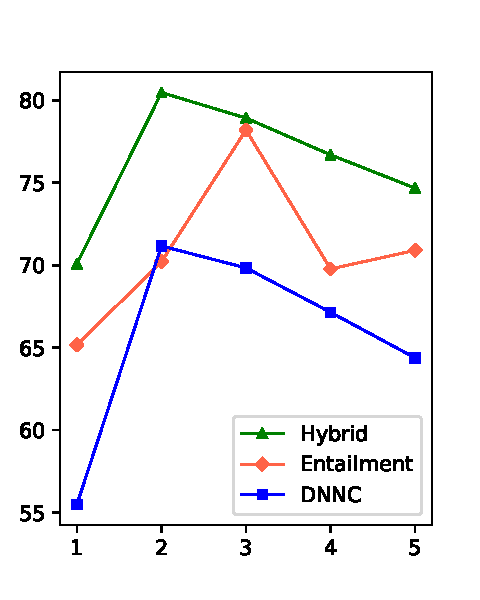
\includegraphics[width=3.8cm]{figure/intent_without_base.pdf}}
\vspace{-0.08in}
\subfigure[\vspace{-0.1in}
\relationdata.]{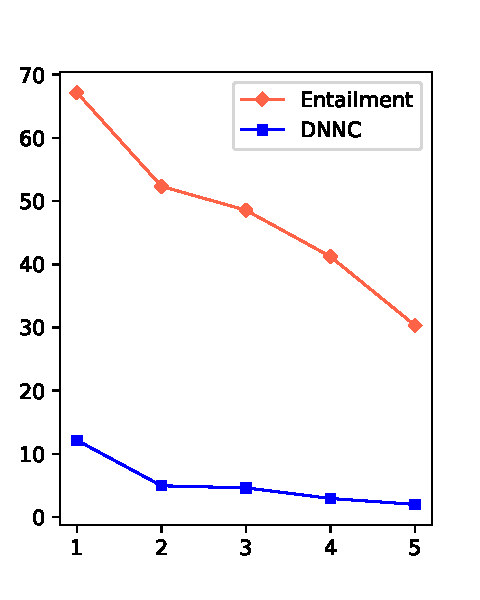
\includegraphics[width=3.8cm]{figure/relation_without_base.pdf}}
\vspace{-0.08in}
\caption{Average performance on new classes in different rounds. The x axis is the number of round and y is the average accuracy on new classes in this round.}
\vspace{-0.1in}
\label{fig:performance_withoutbase}
\end{figure}


\paragraph{Implementation and setting.}
For DNNC, \modelname, and \hybrid , we use the MNLI \cite{williams2018broad} dataset to pre-train these models. 
All systems are implemented through the Huggingface Transformers package.
%\footnote{\url{https://github.com/huggingface/transformers}} 
For both pre-training and fine-tuning, we set the learning rate as 1e-6, the batch size is 16. We run 20 epochs for the pre-training. For the fine-tuning process, we run 5 epochs on \intentdata\enspace and 50 epochs on \relationdata.
%We always fine-tune on each round 5 epochs with learning rate 1e-6 and batch size 16. 
We run the same program with 3 different seeds and report the average performance. Accuracy is reported for \{$C_b$, $C_n^1$, $\cdots$, $C_n^5$\} and F1 score for $C_o$.





\iffalse
\begin{table*}[t]
\setlength{\tabcolsep}{4.5pt}
%  \setlength{\belowcaptionskip}{-5pt}
%  \setlength{\abovecaptionskip}{5pt}
\small
  \centering
  \begin{tabular}{ll|c|c|c|c|c|c|c}
 & & $C_b$ & $C_n^1$ & $C_n^2$ & $C_n^3$ & $C_n^4$ & $C_n^5$ & $C_o$\\\hline\hline
\multirow{5}{*}{$C_b$} & ProtoNet &  \\
  &  Entailment &  \\
  &  Clu4Fewshot &  \\
  & DyFewShot &   & & & & & &  \\
  
  &  \modelname & \\\hline
 \multirow{5}{*}{$C_n^1$} & ProtoNet &  \\
   &  Entailment & \\
  &  Clu4Fewshot &  \\
  & DyFewShot &   &   & & & & &  \\
  &  \modelname &  \\\hline
  
 \multirow{5}{*}{$C_n^2$} & ProtoNet &  \\
    &  Entailment &  \\
  &  Clu4Fewshot  & \\
  & DyFewShot &  \\
  &  \modelname & \\\hline
  
 \multirow{5}{*}{$C_n^3$} & ProtoNet &  \\
 & Entailment &  \\
  &  Clu4Fewshot &  \\
  & DyFewShot &  \\
  &  \modelname&   \\\hline
  
 \multirow{5}{*}{$C_n^4$} & ProtoNet &  \\
 & Entailment & \\
  &  Clu4Fewshot &  \\
& DyFewShot &  \\
  &  \modelname &  \\\hline


 \multirow{5}{*}{$C_n^5$} & ProtoNet &  \\
 & Entailment & \\
  &  Clu4Fewshot  & \\
  & DyFewShot &  \\
  &  \modelname &   \\
\end{tabular}
\caption{System performance on the benchmark \relationdata.}\label{tab:relationresults}
\end{table*}
\fi
\subsection{Experimental results}
As the problem formulation presented in Section \ref{sec:probdefinitino}, we want to investigate two questions. $\mathcal{Q}_1$: can our system get better performance on each round? $\mathcal{Q}_2$: can our system hold more stable performance during the incremental learning process? We answer these questions separately under the incremental learning setting with or without base classes.

\begin{figure}[t]
\centering
\subfigure[Average Performance.]{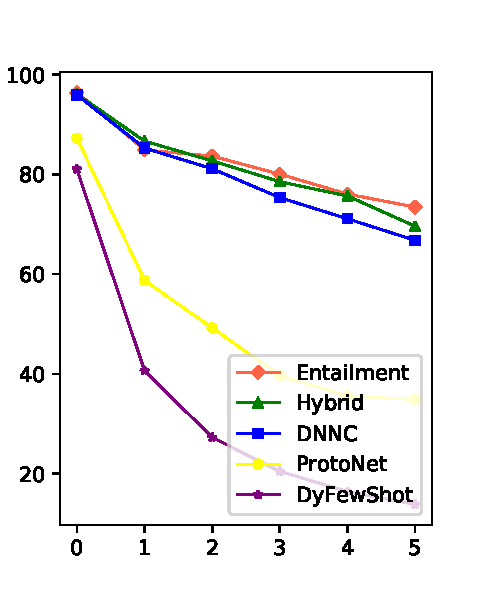
\includegraphics[width=3.8cm]  {figure/intent_with_base.pdf}} \vspace{-0.05in}
\subfigure[Performance drop rate.]{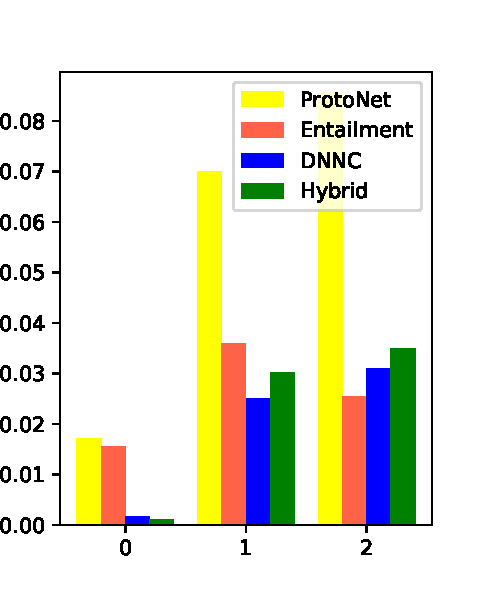
\includegraphics[width=3.8cm]{figure/drop_rate.pdf}} \vspace{-0.05in}
\caption{Performance analysis on \intentdata\enspace with base classes. In Figure (a), X axis is the number of round, where 0 indicates the round of base classes; Y axis is the average performance on all the seen classes in this round (including base classes $C_b$ and new classes $C_n^1$, ..., $C_n^i$). In Figure (b), X axis indicates a subset of classes, where 0 indicates base classes and 1 indicates new classes in $C_n^1$; Y axis is the performance drop rate $d$ for different subsets.}
\label{fig:performance_with_base}
\vspace{-0.05in}
\end{figure}

\paragraph{Incremental learning without base classes.}
Tables \ref{tab:intentresults_withoutbase}$\sim$\ref{tab:relationresults_withoutbase} list the results on two benchmarks, \intentdata\enspace and \relationdata\enspace,  for the setting without base classes, respectively.  For the \intentdata\enspace benchmark, we compare \modelname\enspace with DNNC, together with their hybrid model \hybrid\enspace for 5 rounds. For the \relationdata\enspace benchmark, we only compare \modelname\enspace with DNNC since \hybrid\enspace is not applicable for this dataset. The label (relation type) is not compatible with the input instance (an utterance with an entity pair). Therefore, we can not mix the pairs from these two models (\modelname\enspace and DNNC) to train a hybrid model.

%So we can not mix the pairs from these two models to train a hybrid model.  v As we mentioned in Line 529, the input x and y are not consistent for the relation classification task, therefore HYBRID is not working for this dataset.
%As shown in table \ref{tab:intentresults_withoutbase}, the hybrid model \hybrid\enspace achieves the best performance on most cases. 

As for question $\mathcal{Q}_1$, we find that \modelname\enspace and \hybrid\enspace outperform all the baselines. These results show the effectiveness of formalizing text classification as a textual entailment problem.
%This shows that \modelname\enspace is better than DNNC even they all pre-trained by MNLI.
%which shows the effectiveness of formalizing text classification as a textual entailment problem.
%This means that the pairs generated by \modelname\enspace are better than the pairs used in DNNC. 
For the benchmark \intentdata\enspace, the hybrid model, \hybrid, achieves the best performance since it has the largest number of entailment pairs (by combining pairs from two models) for the training. It shows in the extreme case that no base classes are available, the more data the better. For the benchmark \relationdata, this task is much more difficult compared to intent detection due to the complicity of the training examples (utterances with entity pairs). DNNC does not perform well for this task since comparing two complex examples can not benefit from the pre-training entailment model.

As for $\mathcal{Q}_2$, we show the average performance change on new classes in Figure \ref{fig:performance_withoutbase}. For \intentdata, the average performance of new classes increases in the beginning then drops for the remaining rounds. This might due to the lack of training data in the first found. For \relationdata, the average performance drops dramatically due to this task is much more difficult.
%compared to the pre-training entailment task. 


\paragraph{Incremental learning with base classes.}
The results on \intentdata\enspace with base classes are shown in Table \ref{tab:intentresults}. 
We compare our systems \modelname\enspace and \hybrid\enspace with three baselines: DNNC, ProtoNet, and DyFewShot. This setting is evaluated incrementally on base classes, five rounds of new classes, and OOD.


%Our system \modelname\enspace is compared with the baselines for the seven batches of testing classes (base, five rounds and OOD) along with the incremental learning from the base classes to the fifth round. 


As for question $\mathcal{Q}_1$, we summarize our observations as follows. 
(i) Pre-trained models (\modelname, \hybrid, and DNNC) work much better than few-shot learning methods (ProtoNet and DyFewShot) which means pre-training from a large-scale entailment dataset helps a lot in this setting. (ii) Our proposed models, \modelname\enspace and \hybrid\enspace obtain comparable performances and they outperform all the other baselines consistently in all test classes for the whole timeline. This shows the effectiveness of our proposed method of generating (utterance, label) entailment pairs.

%(iii) Our system \modelname\enspace consistently obtains the best results across all test classes and the timeline.

\iffalse
\begin{table}[t]
\centering
\resizebox{\linewidth}{!}{% <-
\begin{tabular}{l|c|c}
             & {\intentdata} & {\relationdata}\\ \hline
ProtoNet &       25.834     &              \\
Entailment   &            &              \\
Clu4Fewshot      &            &              \\
DyFewShot      &            &              \\
\modelname          &            &             
\end{tabular}
}
\caption{Average performance on new classes in fifth round, $C_n^5$, for two benchmarks.}
\end{table}
\fi






% To answer the question $\mathcal{Q}_2$, we need to quantify the performance changes of all systems  along the timeline not only on $C_b$ but also on all \{$C_n^i$\} ($i=1,\cdots, 5$). Given a list of $m$ result values $r\in\mathbb{R}^m$, we first use linear regression to fit these numbers. For example, if we fine a line $f(x)=a*x+b$, where $a<0$ is the slope,  $b$ is the intercept, and $t=1, \cdots, m$ is the time stamp. The performance drop $d$ reflected by this list is calculated as $d= (f(1)-f(m))/f(1)$. Since the linear regression is more reliable when the $m$ value is larger, we compute the drop values for $C_b$, $C_n^1$ and $C_n^2$ only and average them as the final evaluation of a system in responding to  the question $\mathcal{Q}_2$.

To answer $\mathcal{Q}_2$ in this setting, we propose a new evaluation metric, performance drop rate $d$, to evaluate the performance change along the timeline, i.e., how fast the performance drops when adding new rounds of classes into the system. For example, the performances on base classes decrease when incrementally adding five rounds of new classes into the system. Given a list of performance results for a certain subset of classes (for example, base classes) on $m$ rounds, $r = (r_1, r_2, ..., r_m)$, we calculate the performance drop rate as the average drop rate of different rounds $d =\frac{1}{m-1}  \sum_{i=0}^{m-1} (r_i - r_{i+1}) / r_i $. In the experiments, we calculate $d$ for four methods on base classes, new classes in round1 and round2 separately. The average drop rate of DyFewShot is not reported since there are 0.0 values in the performance. 

In Figure \ref{fig:performance_with_base}, we show the average performance on all the seen classes in different rounds (including base classes and all the seen new classes) in (a) and the performance drop rate $d$ in (b). As shown in Figure \ref{fig:performance_with_base} (a), the average performance drops with the increase of round numbers. We can also observe that our proposed models \modelname\enspace and \hybrid\enspace achieve the best performance on the average performance on all the seen classes, including base classes and new classes.
%As shown in Figure 2, the average performance drops with the increase of round numbers. 
Figure \ref{fig:performance_with_base} (b) shows the the performance drop rate $d$ for different models. ProtoNet and \modelname\enspace have higher drop rate than DNNC and \hybrid\enspace on base classes.
For new classes in round1 and round2, the drop rate on ProtoNet is much higher than all the entailment methods. In summary, \modelname\enspace achieves the best performance on the average accuracy of all seen classes, while DNNC is more stable and has a lower performance drop rate. \hybrid\enspace combines the advantages of both models by combining these two models together.
%we evaluate the performance of base classes when adding five rounds of new classes into the system.

%evaluate the performance change on the base classes given five rounds of new classes.

%Given a list of $m$ result values $r = (r_1, r_2, ..., r_m)$, we calculate the average drop in each round $d =\frac{1}{m-1}  \sum_{i=0}^{m-1} (r_i - r_{i+1}) / r_i $. 





\section{Conclusion}
In this work, we define a new challenge in the NLP domain, incremental few-shot text classification with multi-round new classes in two settings: with or without base classes. In addition to the problem formulation, we also release two benchmark datasets for this particular challenge: \intentdata\enspace and \relationdata. Two approaches, \modelname\enspace and \hybrid\enspace are proposed to solve this problem. They convert the text classification problem into textual entailment and make the maximum utilization of the pre-training textual entailment model. Extensive experiments are conducted and the results consistently show the effectiveness of our proposed models.

\section*{Acknowledgments}
We thank the reviewers for their valuable comments.
This work is supported in part by NSF under grants III-1763325, III-1909323, and SaTC-1930941. 


\bibliography{naacl2021}
\bibliographystyle{acl_natbib}


\end{document}
